\section{Evaluation of Fides Resilience in Different Scenarios}
\label{sec:fides-resilience}

To evaluate the resilience of Fides in different scenarios, we need to find the optimal configuration for the following parameters in Fides: interaction evaluation strategy (Section~\ref{sec:interaction-evaluation-strategies}), threat intelligence aggregation function (Section~\ref{sec:network-intelligence-aggregation}) and initial reputation (Section~\ref{subsubsec:computing-reputation}). Each combination of parameters is evaluated in its capacity to correctly classify targets in \textit{any} network topology.\footnote{Distribution of correct/uncertain/incorrect/malicious peers in the network.}
In other words, what setup should the Fides's administrator use in order for Fides to guarantee that it will be able to \textit{eventually} classify targets correctly.

We discovered that actually there \textbf{exists} a particular setup that guarantees that Fides is able to eventually classify the targets correctly in a very adversarial situation. When Fides communicates with at least 25\% of pre-trusted peers from pre-trusted organizations ($0.25 \cdot |P|$ are pre-trusted) and uses $DistanceBasedTIEvaluation$ (section~\ref{subsec:distance-based-eval}) for evaluating the interactions in combination with $AverageConfidenceTIAggregation$ (Section~\ref{subsec:AverageConfidenceTIAggregation}) for aggregating the threat intelligence; then Fides is able to correctly classify the targets no matter how many adversarial peers are in the network (up to filling the remaining 75\%) or how hard they lie.

\subsection{Correct Target Identification Under Harsh Conditions}
\label{subsec:correct-target-identification-no-matter-what}

The first scenario that was evaluated was when the network has 25\% of pre-trusted peers. Several configurations were simulated, which results are shown in Figure~\ref{fig:performance-all-setups-25-pretrusted}. The goal is to find which 

There are three rows and four columns. Each row contains a single interaction evaluation strategy (Section~\ref{sec:interaction-evaluation-strategies}) and each column contains a single metric that evaluates the behavior of that strategy in the network.
There are three different metrics that evaluate the performance of the Fides's setup and the last graph displays how many confident correct (Section~\ref{subsubsec:confident-correct-peer}) peers there are in the network.
The horizontal axis in each graph measures the environment hardness explained in Section~\ref{subsec:environment-hardness}.
The vertical axis is different for each metric.

As mentioned previously, there are three different metrics.
The first column is a metric measuring target detection performance~(\ref{subsec:target-detection-performance-metric}), the second column is the peers' behavior detection metric~(\ref{subsec:peers-behavior-detection-performance-metric}), and the third column measures the average service trust $st^{kmax}_{i, j}$ for all peers in the simulation.

The last, fourth, column then contains a graph that displays what percentage of peers in the simulation were confident correct~(\ref{subsubsec:confident-correct-peer}) with respect to the environment hardness value~(\ref{subsec:environment-hardness}).
We include it in the graph to allow better visualization of how does the simulation environment looks like with respect to the peer's distribution.

\begin{figure}[hp!]
    \centering
    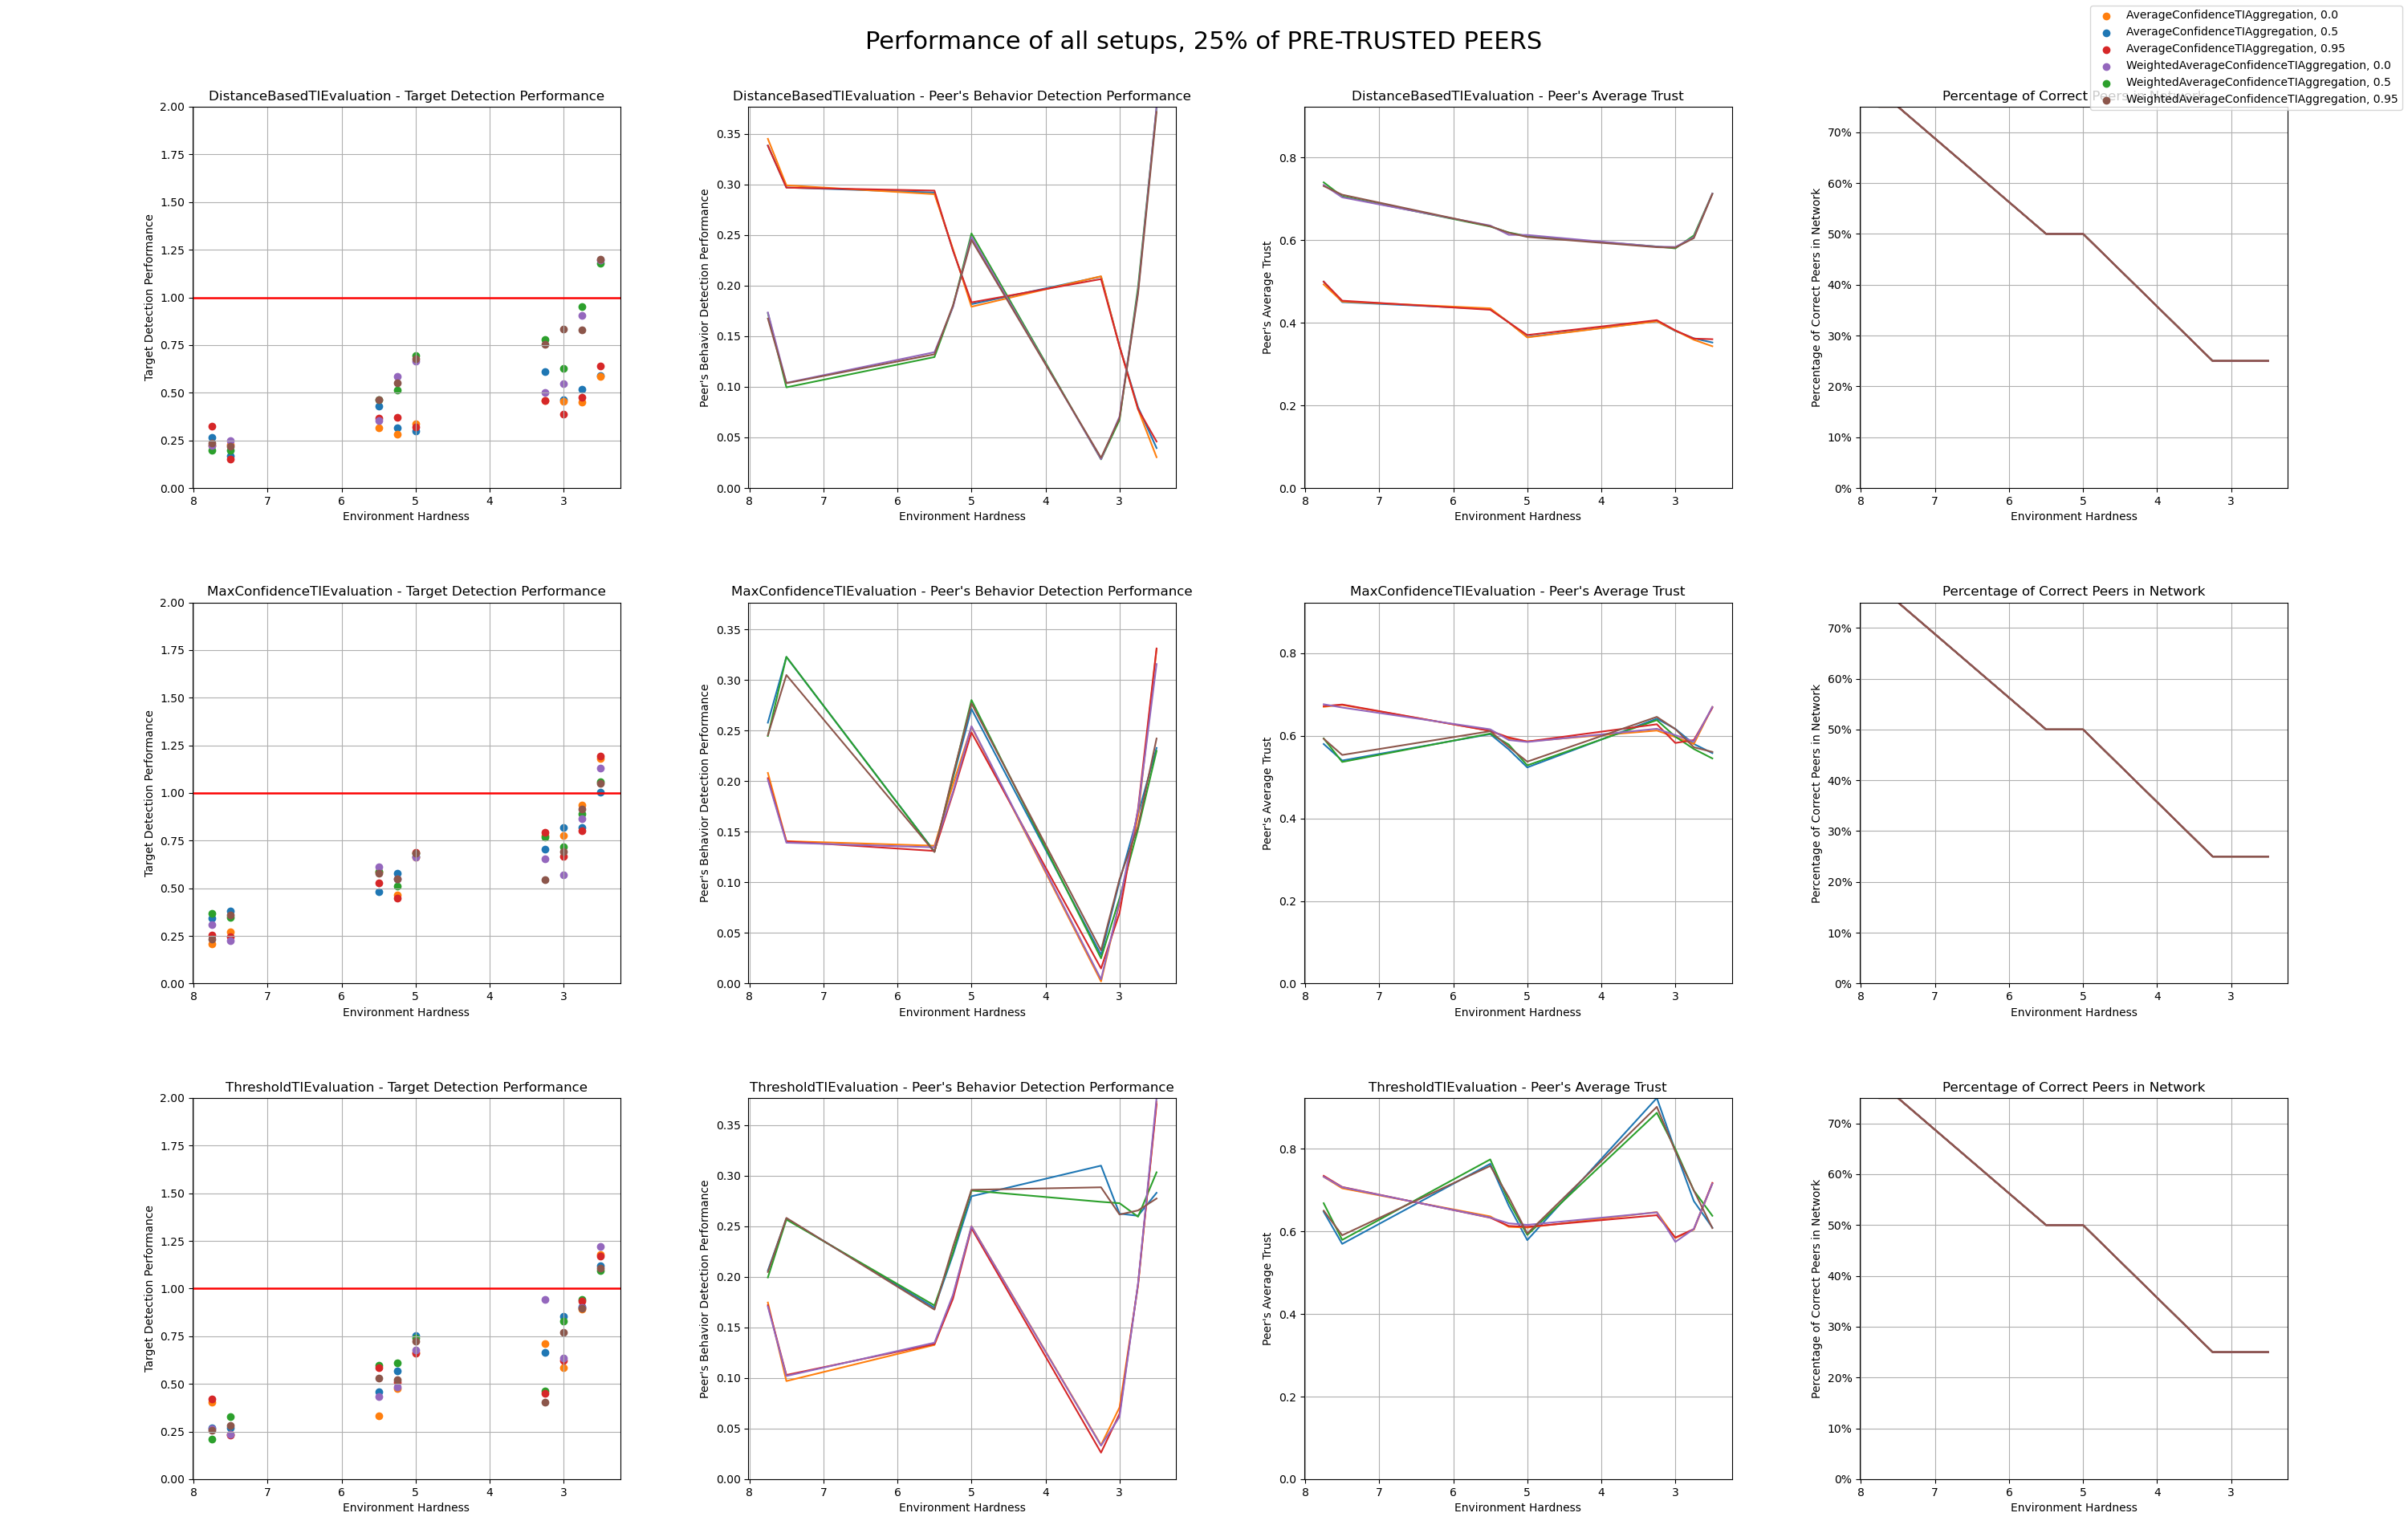
\includegraphics[width=0.94\paperwidth, angle=90]{assets/25_all_metrics.png}
    \caption{Performance of all setups with 25\% pre-trusted peers}
    \label{fig:performance-all-setups-25-pretrusted}
\end{figure}

The most important metric is the target detection performance~(\ref{subsec:target-detection-performance-metric}), which is visualized on the first graph.
A single dot in the graph is the value of $tdp$ and in a case when the $tdp \geq 1$, it means that Fides made on average the wrong decision about the targets and classified them with the wrong label.
In other words, if $tdp \geq 1$, Fides classified benign targets as malicious and the other way around.

\begin{figure}[ht]
    \centering
    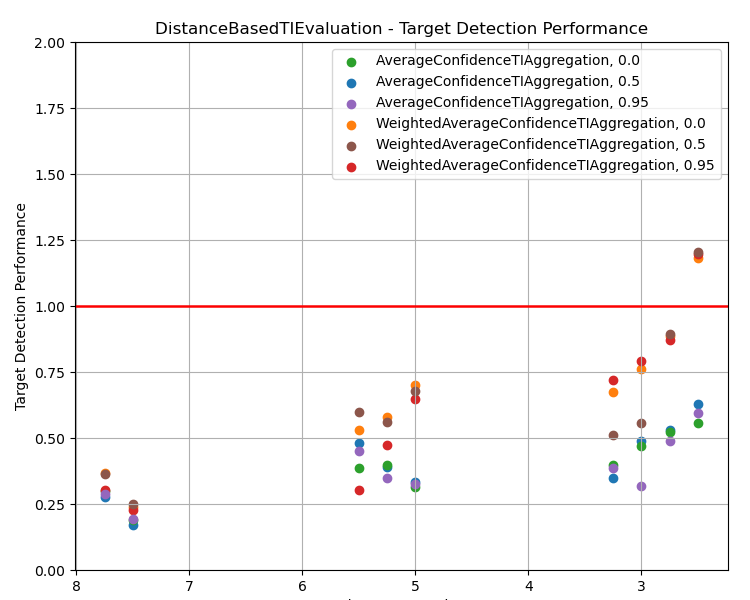
\includegraphics[width=0.7\textwidth]{assets/25_distance_detection_detail.png}
    \caption{$DistanceBasedTIEvaluation$ with 25\% of pre-trusted peers}
    \label{fig:distance-detection-detail-25}
\end{figure}

In Figure~\ref{fig:distance-detection-detail-25} we can clearly see, that there is a situation, even in the hardest environment, where the $DistanceBasedTIEvaluation$ in combination with $AverageConfidenceTIAggregation$ does not have any $tdp$ above the \textit{red line} which means that $tdp < 1$ and that Fides was always able to identify targets correctly even in the worst possible environment.

We included the graph of this case similar to the Figure~\ref{fig:single-simulation-example} with this particular \textit{"winning"} setup in the most hostile environment to the appendix in Figure~\ref{fig:worst-best-scenario}. For the explanation of the graph see Section~\ref{sec:general-overview-of-simulation-output}.

Interestingly, in this particular case, the initial reputation does not affect the final outcome of the simulation, but it does affect the progress as when using an initial reputation higher than $0$, Fides provides wrong scores in the situation when the malicious peers started to lie.
However, it discovers that the peers are lying, which decreases their service trust and is able to eventually recover the correct labels for the targets.
The score value over time for this situation can be seen on the Figure~\ref{fig:missclassification-score-only}.
We included the whole graph in the appendix in Figure~\ref{fig:missclassification-recovery}.

\begin{figure}[ht]
    \centering
    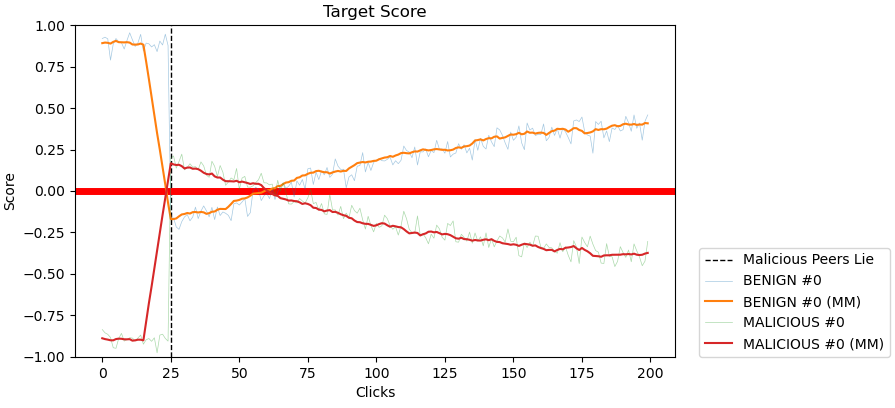
\includegraphics[width=0.9\textwidth]{assets/misclassification_score.png}
    \caption{Score in figure~\ref{fig:missclassification-recovery}.}
    \label{fig:missclassification-score-only}
\end{figure}

It is clear from Figure~\ref{fig:distance-detection-detail-25}, that when Fides used the threat intelligence aggregation method $WeightedAverageConfidenceTIAggregation$~(\ref{subsec:WeightedAverageConfidenceTIAggregation}), it miss-classified the targets in one situation.
Thus, this method does not provide a guarantee that Fides will end up with correct classifications for every target.

The same applies to all other interaction evaluation methods as we can see in the Figure~\ref{fig:performance-all-setups-25-pretrusted} that in the hardest environment, they all classified the targets poorly with all threat intelligence aggregation methods.

\subsection{Scenarios of No pre-trusted peers, and 50\% pre-trusted peers}
\label{subsec:resilience-under-different-conditions}
Other two important scenarios to consider are the situations where the administrator does not have any pre-trusted peers and when at least 50\% of peers are pre-trusted.

With no pre-trusted peers in the network, the results of each configuration vary and they highly depend on the network topology as well as on the knowledge of the local Slips instance. The results for the no pre-trusted scenario are shown in Appendix Figure~\ref{fig:performance-all-setups-0-pretrusted}.


In the scenario of 50\% pre-trusted peers, no matter the configuration, Fides was eventually able to determine the correct target classification with a high precision of $tdp \leq 0.7$. Moreover, Fides was able to correctly identify the peer's behavior with the precision of $pbdp \leq 0.2$. This is a very favorable situation for the administrator, where you trust the peers so much that it is not possible for the adversarial peers to modify the belief. The results for this scenario are shown in Appendix Figure~\ref{fig:performance-all-setups-50-pretrusted}.

